O aprendizado supervisionado é o campo dentro de aprendizado de máquina que visa a gerar modelos preditores a partir de um conjunto de dados de treinamento cujos resultados são previamente conhecidos.

\section{Naive Bayes}

\textit{Naive Bayes} é uma das técnicas mais simples disponíveis nesse contexto. Ela se baseia no teorema de Bayes enquanto assume independência entre as características escolhidas para descrever o dado. Abaixo veremos sua formulação matemática como descrita por Schütze \cite{schutze08}.

Tendo $\mathbf{x}$ tal que $\mathbf{x} \in \mathbf{X}$ em que $\mathbf{X}$ é o conjunto de dados de treinamento, a sua probabilidade de pertencer a classe $c_k \in \mathbf{c}$ é dada pelo teorema de Bayes:
\begin{equation} \label{eq:bayes}
    p(c_k \mid \mathbf{x}) = \frac{p(c_k) \ p(\mathbf{x} \mid c_k)}{p(\mathbf{x})}
\end{equation}

Sendo $\mathbf{x}$ um vetor de $n$ características, ao se assumir independência entre elas obtém-se:
\begin{equation}
    p(x_i \mid x_{i+1}, \dots ,x_{n}, c_k ) = p(x_i \mid c_k)
\end{equation}

Logo, pode-se rescrever a equação~\ref{eq:bayes} substituindo $p(\mathbf{x} \mid c_k)$ pelo produtório de suas características:
\begin{equation}
    p(c_k \mid \mathbf{x}) = \frac{p(c_k) \prod_{i=1}^n p(x_i \mid c_k)}{p(\mathbf{x})}
\end{equation}

Como $p(\mathbf{x})$ será uma constante dado cada exemplo $\mathbf{x}$ esta pode ser desprezada:
\begin{equation}
    p(c_k \mid \mathbf{x}) \propto p(c_k) \prod_{i=1}^n p(x_i \mid c_k)
\end{equation}

Portanto, tem-se que o estimador ótimo $\hat{y}$ escolherá pela classe que atinja maior probabilidade:
\begin{equation}
    \hat{y} = \underset{k \in \{1, \dots, K\}}{\operatorname{max}} \ p(c_k) \displaystyle\prod_{i=1}^n p(x_i \mid c_k)
\end{equation}

Vê-se então que o modelo de \textit{Naive Bayes} depende apenas de $p(c_k)$ e $p(\mathbf{x} \mid c_k)$. Estes parâmetros serão extraídos do conjunto de treino por máxima verosimilhança.

Dado um vetor $\mathbf{y}$ de tamanho $m$ que representa as classificações referentes a $\mathbf{X}$, pode-se estimar $p(c_k)$ pela contagem de vezes que a classe $c_k$ aparece no conjunto de treinamento:
\begin{equation}
    \hat{p}(c_k) = \frac{\sum_{i=1}^m [y_i = c_k]}{m}
\end{equation}

Por sua vez, $p(x_r \mid c_k)$ é estimado utilizando a contagem de vezes que uma característica aparece dividida pelo total de características presentes em $\mathbf{X'}$ que é o subconjunto de treino pertencente a classe $c_k$:
\begin{equation}
    \hat{p}(x_r \mid c_k) = \frac{\sum_{j=i}^{m'} \sum_{i=1}^n [x_{ji} = x_r]}{|\mathbf{X'}|}
\end{equation}

Vê-se que modelos montados a partir de \textit{Naive Bayes} são computacionalmente baratos dado que seus parâmetros são obtidos através de contagens sobre os dados de treinamento e que sua predição utiliza apenas multiplicações.
Embora se baseie na independência entre características, seu baixo custo operacional leva esta técnica a ser utilizada mesmo em problemas com notória dependência de características como a classificação de texto \cite{mccallum98}.

\section{Support Vector Machine}

O conceito fundamental do \textit{Support Vector Machine} (SVM) se dá pela obtenção de um vetor de suporte que melhor separe as classes. Esta separação é feita de maneira que se maximize a margem entre as classes. A figura~\ref{fig:svm} demostra dados de duas classes distintas, representadas pelas cores rosa e amarelo, pertencentes a um espaço de características de duas dimensões; vê-se na figura que a reta que define a maior separação é suportada pelos dados de cada classe mais próximos a ela.

\begin{figure}
\begin{center} {
    \begin{center}
    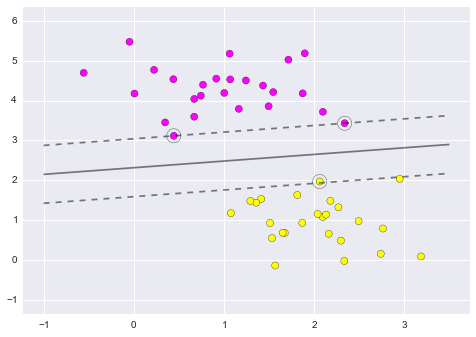
\includegraphics[scale=0.7]{svm.png}
    \caption{Reta de maior margem entre classes.}
    \small Imagem com direitos cedidos para uso não comercial, retirada de \cite{vanderplas15}
    \label{fig:svm}
    \end{center}
}
\end{center}
\end{figure}

Por se basear nos dados próximos ao limiar de separação das classes, o algoritmo passa a ser incapaz de distinguir os casos de classes que não são separáveis sem erros. A solução desse problema foi a criação de uma variável de relaxamento que define um número máximo de erros de classificação permitido. Esta propriedade é descrita com mais detalhes por Cortes e Vapnik em \cite{cortes95}. Sua utilização permite o desenvolvimento de modelos mais robustos a \textit{outliers} e melhora a generalização. Outros exemplos de regularizadores, como este, serão apresentados na subseção~\ref{sec:generalizacao}.

Como utilizam vetores de suporte para definir hiperplanos de separação, SVMs não são capazes de segregar classes não linearmente distinguíveis. Podemos observar um exemplo deste caso na figura~\ref{fig:svm-lin}, na qual um SVM treinado tenta separar classes concêntricas.

\begin{figure}
\begin{center} {
    \begin{center}
    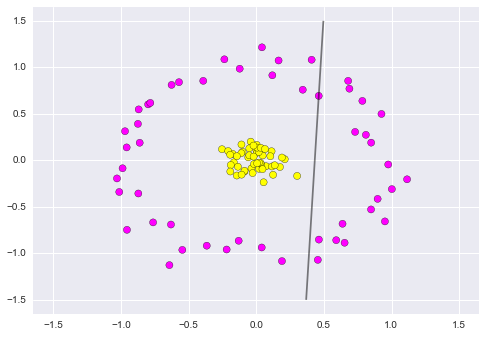
\includegraphics[scale=0.7]{svm-lin.png}
    \caption{SVM em dados não linearmente separáveis.}
    \small Imagem com direitos cedidos para uso não comercial, retirada de \cite{vanderplas15}
    \label{fig:svm-lin}
    \end{center}
}
\end{center}
\end{figure}

Para contornar esse impedimento, foi elaborado o que se chamou de \textit{kernel trick}. Este se baseia em um mapeamento não linear dos dados para um espaço onde possam ser linearmente separáveis \cite{scholkopf02}. A figura~\ref{fig:svm-rbf} mostra a representação dos dados apresentados na figura~\ref{fig:svm-lin} após seu mapeamento por uma função de base radial.

\begin{figure}
\begin{center} {
    \begin{center}
    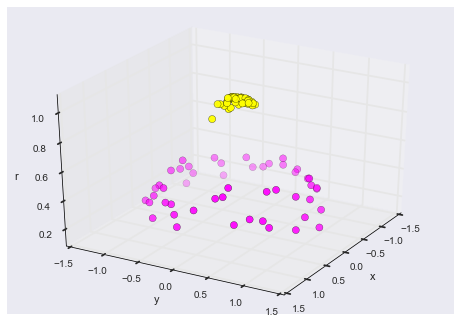
\includegraphics[scale=0.7]{svm-rbf.png}
    \caption{Transformação de dados por função de base radial.}
    \small Imagem com direitos cedidos para uso não comercial, retirada de \cite{vanderplas15}
    \label{fig:svm-rbf}
    \end{center}
}
\end{center}
\end{figure}

Neste novo espaço definido pela transformação, os dados são linearmente separáveis. Portanto, é possível achar um vetor de suporte que defina um hiperplano de separação das classes. Vemos na figura~\ref{fig:svm-rbf-clas} as margens encontradas.

\begin{figure}
\begin{center} {
    \begin{center}
    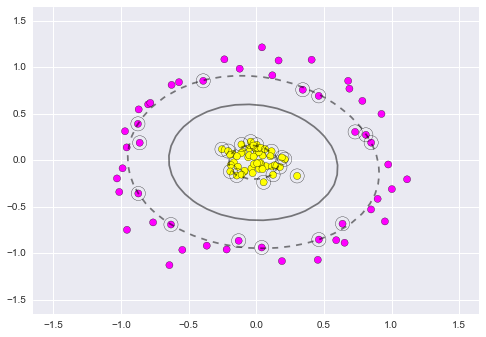
\includegraphics[scale=0.7]{svm-rbf-clas.png}
    \caption{SVM com \textit{kernel} de base radial.}
    \small Imagem com direitos cedidos para uso não comercial, retirada de \cite{vanderplas15}
    \label{fig:svm-rbf-clas}
    \end{center}
}
\end{center}
\end{figure}

Uma limitação na utilização deste algoritmo é seu tempo de treinamento. Sua complexidade computacional fica entre $O(n_{caracteristicas} \times n_{dados}^2)$ e $O(n_{caracteristicas} \times n_{dados}^3)$ \cite{list09}. Porém, Suykens e Vandewalle desenvolveram uma função custo através da qual tornou possível realizar o treinamento de SVMs a partir da otimização pelo método do gradiente \cite{suykens99}.

\section{Redes Neurais} \label{sec:nn}

redes neurais são sistemas computacionais que visam replicar o modelo de processamento do cérebro. Há diversas variações de redes neurais. Nesta subseção será abordada a mais simples, redes neurais feedforward, e na subseção~\ref{sec:convolucionais} serão apresentadas redes neurais Convolucionais.

Redes neurais feedforward são compostas de camadas de neurônios sucessivamente interligadas por sinapses. As sinapses funcionam como um ponderador linear dos neurônios da camada anterior. Os neurônios, por sua vez, representam uma função de ativação, normalmente não linear, tais como: tangente hiperbólica, logística etc. Como exemplificação, há a figura~\ref{fig:ff-neural-net}, onde apresenta-se o diagrama de uma rede que conta com uma camada de entrada que representa os dados do problema, seguida de duas camadas intermediarias, comumente chamadas de escondidas, as quais são seguidas pela camada de saída, que apontará o resultado final de todo processamento da rede.

\begin{figure}
\begin{center} {
    \begin{center}
    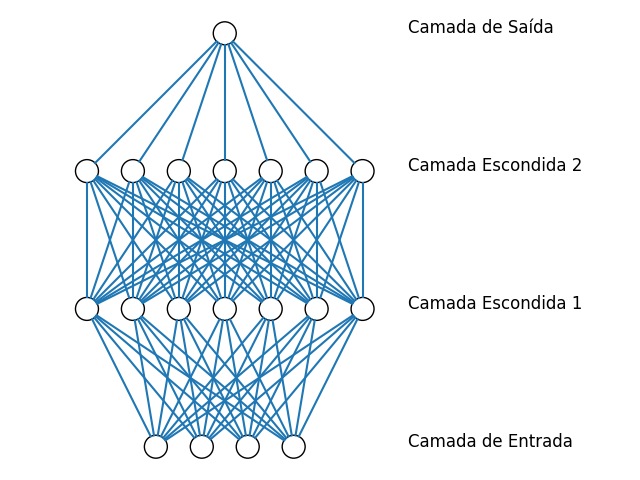
\includegraphics[scale=0.75]{ffnn.png}
    \caption{Rede Neural Feedforward}
    \label{fig:ff-neural-net}
    \end{center}
}
\end{center}
\end{figure}

Uma de suas principais características de redes neurais é a capacidade de aproximar qualquer função, dado que a rede contenha pelo menos uma camada escondida com número suficientemente grande de neurônios com ativação não linear \cite{hornik89}.

Para uma Rede Neural simular uma função, precisa-se obter o conjunto de pesos, ou sinapses, que torne esta rede uma boa representação para a função escolhida. Em outras palavras, precisa-se minimizar o erro da representação da rede dado que este erro é uma função das sinapses. Uma prática comum é inicializar a rede com pesos selecionados de uma distribuição uniforme com média zero e desvio padrão inversamente proporcional ao número de dados de treinamento \cite{lecun12}. Posteriormente, é feita uma otimização da representação em função dos pesos. Para realizar esta otimização, utiliza-se normalmente \textit{Backpropagation} para se encontrar o ajuste ideal de cada sinapse baseada, em sua contribuição no erro. Uma explicação deste método é apresentada por Williams e Hinton em \cite{williams86}.

\subsection{Deep Learning}

O sucesso na aplicação de redes neurais nas mais diversas áreas levou à utilização de redes cada vez mais robustas. Assim, redes neurais profundas romperam barreiras de performance em problemas como reconhecimento de fala, detecção de objetos, tradução etc \cite{lecun15}. Chamou-se de \textit{Deep Learning} o campo de estudo de redes neurais com muitas camadas.

Cada camada de uma Rede Neural gera uma abstração que representa a sua entrada de modo a facilitar a tarefa a ser realizada. O encadeamento de camadas resulta em representações mais complexas dos dados, revelando relações previamente não observáveis. O aprofundamento das redes visa a reduzir ou eliminar a chamada \textit{feature engineering}, processo de seleção de características, que usualmente requer expertise no domínio do problema. Considerando por exemplo o caso do diagnóstico de câncer de pele, técnicas tradicionais de classificação dependiam de extração de informações de imagens de lesões, tais como: formato, tamanho, cor etc. Modelos baseados em redes neurais profundas são capaz de obter resultados superiores, eliminando completamente esta etapa \cite{esteva17}.

\subsection{Redes Neurais Convolucionais} \label{sec:convolucionais}

A utilização de redes neurais feedforward em imagens sofre limitações, por cada pixel estar diretamente ligado aos neurônios, rotações ou translações na imagem afetam fortemente a capacidade da rede. Pretendendo solucionar estes problemas, foram desenvolvidas redes neurais Convolucionais, cujas conexões são baseadas no funcionamento do córtex visual.

Elas são compostas primariamente de dois tipos de camadas: convolucionais e \textit{pooling}. Camadas convolucionais são formadas por um conjunto de filtros espaciais compostos das mesmas funções não-lineares utilizadas em Redes feedforward \cite{goodfellow16}. Para cada exemplo do conjunto de dados, o filtro, cujo tamanho é menor que a entrada, é aplicado no inicio do dado e deslocado até o final. Desta forma, os filtros dividem os pesos entre todo espaço do dado, permitindo uma insensibilidade a deslocamentos e rotações. Por sua vez, as camadas de \textit{pooling} visam reduzir o número total de sinapses da rede. Para tal, reduz-se o tamanho dos filtros, obtendo-se valores máximos ou médias de dimensões desses filtros. \textit{Pooling} é fundamental quando o objetivo a ser atingido depende mais da presença de uma característica do que sua sua posição no dado \cite{goodfellow16}.

Por fim, apesar de Redes Convolucionais terem sido desenvolvidas com intuito de solucionar problemas de visão computacional, elas também obtiveram êxito nas mais diversas áreas, como no reconhecimento de voz e em séries temporais \cite{lecun95}. Tal sucesso pode ser atribuído à insensibilidade da rede a deslocamentos.

\section{Funções Custo} \label{sec:custo}

Dá-se o nome de \textit{função custo} às funções que caracterizam a distância entre o resultado obtido pela rede e seu objetivo. Assim, as sinapses de redes neurais são otimizadas a partir da minimização de tais funções. Nesta seção, serão apresentadas as funções custo mais relevantes no contexto de redes neurais.

\subsection{Erro Médio Quadrático}

A função custo mais utilizada é o erro médio quadrático (EMQ). Seu fator quadrático pune mais severamente grandes erros, acelerando o processo de otimização.

A fórmula~\ref{eq:mse} mostra a composição do EMQ sendo $n$ o número de pares de exemplos e $\hat{y}$ a predição da rede neural.

\begin{equation} \label{eq:mse}
    \frac{\displaystyle\sum^n |\hat{\mathbf{y}}_i - \mathbf{y}_i|^2}{n}
\end{equation}

\subsection{Erro Médio Absoluto}

O erro médio absoluto se assemelha ao EMQ, tendo como diferença a falta do fator quadrático, conforme observa-se na fórmula~\ref{eq:mae}.

\begin{equation} \label{eq:mae}
    \frac{\displaystyle\sum^n |\hat{\mathbf{y}}_i - \mathbf{y}_i|}{n}
\end{equation}

\subsection{Erro Médio Absoluto Percentual}

Há situações em que se pretende mapear um objetivo com extensão de diferentes ordens de grandeza. O uso de erro médio quadrático ou absoluto nestes casos irá dar menos relevância a entradas pequenas. Para solucionar este problema, o erro médio absoluto percentual é composto conforme apresentado na fórmula~\ref{eq:mape}

\begin{equation} \label{eq:mape}
    \frac{100}{n}\sum^n \left|\frac{\hat{\mathbf{y}}_i - \mathbf{y}_i}{\mathbf{y}_i}\right|
\end{equation}

\subsection{Entropia Cruzada}

A entropia cruzada é uma medida que contém a distância entre duas distribuições de probabilidades. Sua formula é disposta de maneira que sua otimização encontre os parâmetros de máxima verossimilhança. As equações~\ref{eq:likelihood-label} e~\ref{eq:likelihood-map} mostram a dedução da função de verossimilhança $\mathcal{L}$ a partir da probabilidade a posteriori, na qual $k$ representa cada classe presente no conjunto de dados.

\begin{equation} \label{eq:likelihood-label}
    \mathcal{L}(\theta) = \prod_k P(\mathbf{y}_k \mid \mathbf{x})
\end{equation}

\begin{equation} \label{eq:likelihood-map}
    \mathcal{L}(\theta) = \prod_k \mathbf{\hat{y}}_k^{\mathbf{y}_k} (1 - \mathbf{\hat{y}}_k)^{(1 - \mathbf{y}_k)}
\end{equation}

Para simplificar o custo computacional, o valor máximo da função verossimilhança é obtido minimizando-se o negativo de seu logaritmo, como presente na fórmula~\ref{eq:loglikelihood}.

\begin{equation} \label{eq:loglikelihood}
        -\ln(\mathcal{L}(\theta)) = -\sum_k \mathbf{y}_k \ln(\mathbf{\hat{y}}_k) + (1 - \mathbf{y}_k) \ln(1 - \mathbf{\hat{y}}_k)
\end{equation}

A expressão~\ref{eq:cec} mostra o uso da entropia cruzada como função custo. A segunda parte do somatório determina que a acurácia de não classe pode ser ignorada para determinada classe $k$, visto que esta já será considerada na sua classe correta. É necessário notar que a sua utilização depende de $\mathbf{y}_i$ e $\hat{\mathbf{y}_i}$ serem limitados entre 0 e 1. Para adequar-se a esta limitação, caso a rede neural possua apenas uma saída, utiliza-se ativação Sigmoid na última camada. Em caso de múltiplas saídas, utiliza-se ativação Softmax.

\begin{equation} \label{eq:cec}
    \frac{-\displaystyle\sum^n \sum_k \mathbf{y}_k \ln(\mathbf{\hat{y}}_k)}{n}
\end{equation}

\section{Otimizadores}

Definidas as funções custo, nesta seção serão abordados os algoritmos responsáveis por sua minimização. Embora a área de otimização apresente uma vasta gama de opções, sua utilização em aprendizado de máquina costuma se restringir a algoritmos de primeira ordem, como o gradiente descendente, principalmente por seu menor custo computacional. O método do gradiente, primeiramente apresentado por Cauchy em 1847 \cite{cauchy1847}, consiste em minimizar a função custo por meio de atualizações iterativas de parâmetros do modelo, a partir da derivada da própria função custo em relação aos parâmetros.

Redes neurais, em geral, possuem funções custo não convexas. Assim sendo, o algoritmo de gradiente descendente não garante convergência ao mínimo global. A convergência a mínimos locais torna o modelo sensível a parâmetros, como funções de ativação, número de neurônios, etc., e o torna sensível também à inicialização dos pesos, como mostra Glorot no artigo em que apresenta um método de inicialização de pesos homônimo \cite{glorot10}. Entretanto, o problema de convergência não se limita a mínimos locais. Dauphin \cite{dauphin14} mostra que quanto maior o número de variáveis latentes do modelo, maior a proporção de pontos de sela em relação a mínimos locais. Mostra também que os mínimos locais estão mais propensos a aparecer em pontos críticos com baixo custo, enquanto pontos de sela costumam aparecer em pontos de alto custo. Goodfellow \cite{goodfellow14} apresenta resultados empíricos da efetividade do método do gradiente na fuga dos pontos de sela.

O algoritmo~\ref{al:gd} descreve a forma tradicional do gradiente descendente, dado que $L$ é a função custo adotada e que $\mathbf{\hat{y}}$ é o mapeamento obtido pela rede neural a partir dos dados $\mathbf{x}$ e pesos $\boldsymbol{\theta}$. Observa-se que $\mathbf{\hat{g}}$ é a estimativa do gradiente dos pesos obtida a partir dos dados de treinamento.

\begin{algorithm}
    \caption{Gradiente Descendente}
    \label{al:gd}
    \begin{algorithmic}
        \Require Taxa de treinamento $\epsilon$
        \Require Pesos iniciais $\boldsymbol{\theta}_{0}$
        \Require Número de iterações $T$

        \State $t \gets 0$
        \While {$t < T$}
            \State $t \gets t + 1$
            \State $\mathbf{\hat{y}} \gets f(\mathbf{x}, \boldsymbol{\theta}_{t-1})$
            \State $\mathbf{\hat{g}} \gets \frac{1}{n} \nabla_{\boldsymbol{\theta}} \sum_i^n L(\mathbf{\hat{y}}^{(i)}, \mathbf{y}^{(i)})$
            \State $\boldsymbol{\theta}_{t} \gets \boldsymbol{\theta}_{t-1} - \epsilon \mathbf{\hat{g}}$
        \EndWhile
    \end{algorithmic}
\end{algorithm}

Serão apresentadas nas próximas subseções as variações do método do gradiente mais notórias no treinamento de redes neurais.

\subsection{Gradiente Descendente Estocástico}

    A forma canônica do algoritmo do gradiente descendente começa a apresentar dificuldades de utilização em conjuntos de dados de tamanho considerável. Como observa-se no algoritmo~\ref{al:gd}, para cada atualização dos pesos $\boldsymbol{\theta}$ é necessária a estimação do gradiente $\mathbf{\hat{g}}$, a qual, por sua vez, depende da computação da função custo sobre todos os dados. Além do alto custo computacional, bases de dados grandes tendem a conter várias instâncias de dados muito próximos, não adicionando significativamente informação à estimação do gradiente.

Uma das soluções deste problema, abordada pelo \textit{Gradiente Descendente Estocástico}, é a divisão do conjunto de treinamento em lotes, nos quais serão estimados os gradientes. Cada interação sobre o conjunto inteiro de dados é chamada de época e entre cada época costuma-se embaralhar os dados. Já as outras partes do algoritmo permanecem iguais à implementação tradicional como apresentado em~\ref{al:gd}.

\subsection{Gradiente Descendente com Momento}

A escolha da taxa de treinamento envolve uma troca entre tempo de treinamento e grau de convergência. Altas taxas de treinamento podem apresentar dificuldades de convergência ou comportamentos oscilatórios em torno de um ponto de custo mínimo, enquanto baixas taxas de treinamento consomem muito tempo de treinamento em regiões de alto custo, diminuindo assim sua viabilidade. Objetivando-se obter um melhor compromisso, foi acrescentado o momento ao método do gradiente, como formulado no algoritmo~\ref{al:gdm}. O termo adicional $\mathbf{v}$ representa a "velocidade" do gradiente e a constante de momento $\alpha$ condiz com a taxa de decaimento exponencial do termo $\mathbf{v}$.

\begin{algorithm}
    \caption{Gradiente Descendente com Momento}
    \label{al:gdm}
    \begin{algorithmic}
        \Require Taxa de treinamento $\epsilon$
        \Require Constante de momento $\alpha$
        \Require Pesos iniciais $\boldsymbol{\theta}_{0}$
        \Require Número de iterações $T$

        \State $t \gets 0$
        \State $\mathbf{v}_{0} \gets \vec{0}$
        \While {$t < T$}
            \State $t \gets t + 1$
            \State $\mathbf{\hat{y}} \gets f(\mathbf{x}, \boldsymbol{\theta}_{t-1})$
            \State $\mathbf{\hat{g}} \gets \frac{1}{n} \nabla_{\boldsymbol{\theta}} \sum_i^n L(\mathbf{\hat{y}}^{(i)}, \mathbf{y}^{(i)})$
            \State $\mathbf{v}_{t} \gets \alpha \mathbf{v}_{t-1} - \epsilon \mathbf{\hat{g}}$
            \State $\boldsymbol{\theta}_{t} \gets \boldsymbol{\theta}_{t-1} + \mathbf{v}_t$
        \EndWhile
    \end{algorithmic}
\end{algorithm}

O momento permite que, enquanto o gradiente $\mathbf{\hat{g}}$ mantiver o mesmo sinal entre iterações, o módulo da velocidade $\mathbf{v}$ cresça, acelerando o processo de aprendizado. Quando o sinal do gradiente for invertido, ou seja, passar de um ponto de custo mínimo, o módulo da velocidade será reduzido até seu sentido ser revertido, voltando ao mínimo. Segundo Haykin \cite{haykin09}, o uso do momento tem um efeito estabilizador no algoritmo de aprendizado.

\subsection{Adam}

Outra abordagem adotada nos algoritmos de otimização é o ajuste da taxa de aprendizado de maneira independente para cada dimensão do espaço. Duchi \textit{et al.} \cite{duchi11} propuseram o algoritmo \textit{AdaGrad} (\textit{Adaptative Gradient}), no qual a regra de atualização dos pesos é inversamente proporcional à soma do gradiente ao quadrado em todas iterações anteriores. Dessa forma, direções que tenham grandes e frequentes atualizações serão amortecidas rapidamente, enquanto dimensões com raras atualizações mantêm seu treinamento significativo por mais iterações. Algoritmos com taxa de treinamento adaptativo, como o proposto por Duchi \textit{et al.}, atingem bons resultados em problemas com dimensões esparsas, como o exemplo de Pennington \textit{et al.} \cite{pennington14} no treinamento de \textit{embeddings} de palavras, técnica que será apresentada na seção~\ref{sec:w2v}.

Kingma e Ba \cite{kingma14} projetaram o algoritmo \textit{Adam} \textit{adaptative moment estimation} baseado nos princípios do \textit{AdaGrad}. \textit{Adam} estima o primeiro e segundo momentos do gradiente, média e variância não centralizada, a partir da média móvel de ambos. A regra de atualização de pesos é controlada pela taxa de treinamento $\epsilon$, e pelas estimativas de média e variância, $\mathbf{\hat{m}}$ e $\mathbf{\hat{v}}$ respectivamente, dada a fórmula $\boldsymbol{\theta}_{t} \gets \boldsymbol{\theta}_{t-1} - \epsilon \frac{\mathbf{\hat{m}}_{t}}{\sqrt{\mathbf{\hat{v}}_{t}}} $. Portanto, gradientes grandes por seguidas iterações aumentam a média e, por consequência, o tamanho do passo. Por sua vez, altas variâncias forçam a diminuição da taxa efetiva de aprendizado.

O algoritmo~\ref{al:adam} possui a implementação de \textit{Adam} em pseudocódigo. Os valores dos decaimentos betas costumam ser escolhidos em torno de 0.9 para $\beta_{1}$ e 0.999 para $\beta_{2}$. Pelos momentos serem inicializados em zero, é necessário corrigir a tendência para se obter a verdadeira estimativa.

\begin{algorithm}
    \caption{Adam}
    \label{al:adam}
    \begin{algorithmic}
        \Require Taxa de treinamento $\epsilon$
        \Require Constante de decaimento $\beta_{1}, \beta_{2}$
        \Require Pesos iniciais $\boldsymbol{\theta}_{0}$
        \Require Número de iterações $T$

        \State $t \gets 0$
        \State $\mathbf{m}_{0} \gets \vec{0}$
        \State $\mathbf{v}_{0} \gets \vec{0}$
        \While {$t < T$}
            \State $t \gets t + 1$
            \State $\mathbf{\hat{y}} \gets f(\mathbf{x}, \boldsymbol{\theta}_{t-1})$
            \State $\mathbf{\hat{g}} \gets \frac{1}{n} \nabla_{\boldsymbol{\theta}} \sum_i^n L(\mathbf{\hat{y}}^{(i)}, \mathbf{y}^{(i)})$
            \State $\mathbf{m}_{t} \gets \beta_{1} \mathbf{m}_{t-1} + (1 - \beta_{1}) \mathbf{\hat{g}}$
            \State $\mathbf{v}_{t} \gets \beta_{2} \mathbf{v}_{t-1} + (1 - \beta_{2}) \mathbf{\hat{g}}^{2}$
            \State $\mathbf{\hat{m}}_{t} \gets \frac{\mathbf{m}_{t}}{(1 - \beta_{1}^{t})}$
            \State $\mathbf{\hat{v}}_{t} \gets \frac{\mathbf{v}_{t}}{(1 - \beta_{2}^{t})}$
            \State $\boldsymbol{\theta}_{t} \gets \boldsymbol{\theta}_{t-1} - \epsilon \frac{\mathbf{\hat{m}}_{t}}{\sqrt{\mathbf{\hat{v}}_{t}}} $
        \EndWhile
    \end{algorithmic}
\end{algorithm}

\textit{Adam} apresenta robustez à escolha da taxa de treinamento $\epsilon$, visto que esta funciona como um limite superior da taxa efetiva de atualização dos pesos, como provado em seu artigo \cite{kingma14}, juntamente com sua análise de convergência e com seus resultados experimentais. Por se utilizar de médias móveis na estimação dos momentos, o algoritmo apresenta outra vantagem, sua capacidade de se adaptar a funções objetivos não estacionárias.

Por sua robustez à escolha de hiperparametros e por sua aceleração do processo de aprendizado \textit{Adam} se tornou uma das principais técnicas de otimização de redes neurais profundas.

\section{Generalização} \label{sec:generalizacao}

Um dos principais fatores de um sistema de aprendizado de maquina é sua capacidade de generalizar, isto é, quando seu desempenho em dados de teste, ou seja, dados que não foram utilizados na fase de treinamento, é equivalente ou suficientemente próximo ao obtido durante aprendizado.

A fase de aprendizado do sistema pode ser vista como o processo de ajuste de parâmetros. Desta forma, ao tentar representar a função, o modelo pode sofrer com sobreajuste, \textit{overfitting}, adequando-se demais aos dados de treinamento. O oposto também acontece quando o modelo é incapaz de mapear a complexidade entre as entradas e a saída; a este evento dá-se o nome de subajuste, \textit{underfit}. Tais eventos estão exemplificados na figura~\ref{fig:fitting}.


\begin{figure}
\begin{center} {
    \begin{center}
    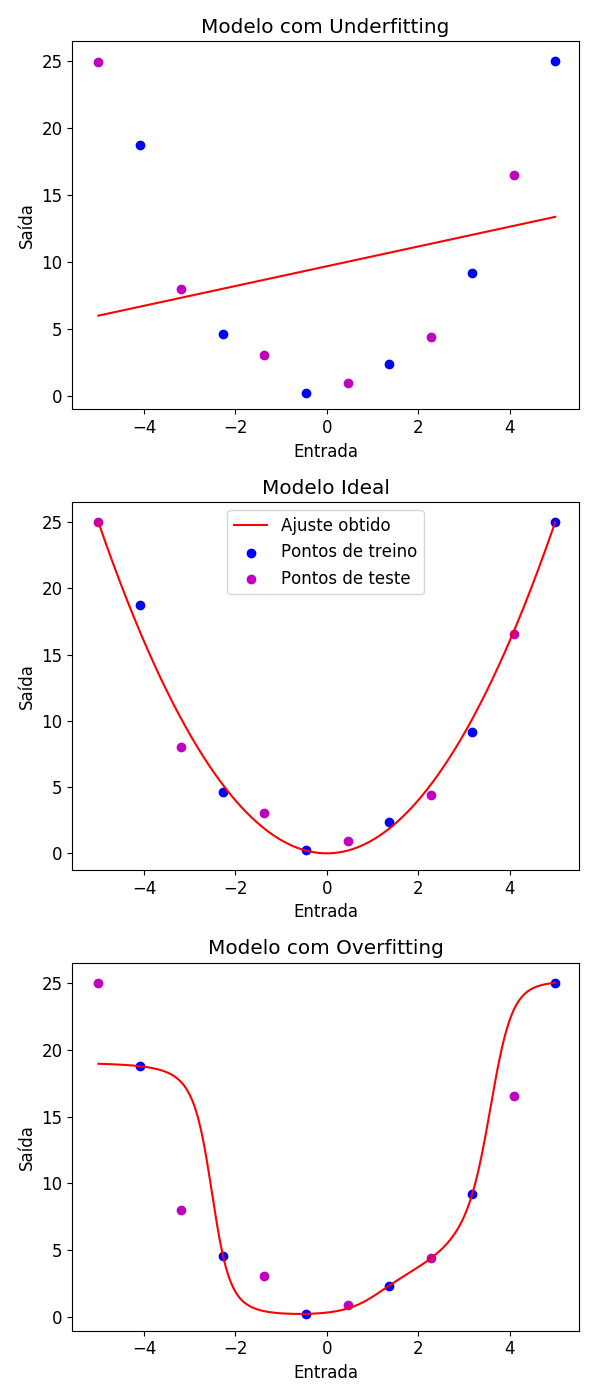
\includegraphics[scale=0.4]{fitting.png}
    \caption{Diferentes pontos de ajuste.}
    \label{fig:fitting}
    \end{center}
}
\end{center}
\end{figure}

O uso de modelos robustos como os de \textit{Deep Learning} implica em uma maior propensão de se obter \textit{overfitting} durante o treinamento, resultado de seu crescente número de parâmetros livres. Abordando esse problema, foi desenvolvido um conjunto de técnicas que visam a reduzir o \textit{overfitting}, conjunto esse que recebe o nome de regularização. Nas subseções seguintes serão apresentadas as duas principais técnicas de regularização.

\subsection{Regularização de Tikhonov}

As regularizações de norma compõem um dos grupos mais simples de regularização. Seu funcionamento é possível pois se adiciona à função custo um termo proporcional aos pesos, penalizando neurônios com grandes normas. Assim, limita-se a capacidade do modelo e, consequentemente, diminui-se o potencial de \textit{overfitting}.

Também conhecida como regularização $L_{2}$, a regularização de Tikhonov utiliza-se da norma quadrática dos pesos. A formula \ref{eq:custo-l2} exemplifica a função custo erro médio quadrático com o termo adicional de regularização $L_{2}$, que por sua vez é controlado por uma constante $\lambda$.

\begin{equation} \label{eq:custo-l2}
    \frac{\displaystyle\sum^n |\hat{\mathbf{y}}_i - \mathbf{y}_i|^2}{n} + \frac{\lambda}{2} \lVert \boldsymbol{\theta} \rVert_{2}^{2}
\end{equation}

Krogh e Hertz \cite{krogh92} provam que o uso de regularização $L_{2}$ é capaz de suprimir parâmetros irrelevantes, diminuindo o número de parâmetros do modelo, e de reduzir o efeito de ruídos presentes na anotação dos dados.

\subsection{Dropout}

\section{Supervisão Distante}
